\section{Time Synchronization}
\label{sec-timesynchronization}
\label{subsec-multihoptimesync}

Unlike the sensor interface board, in which a simple prototype led directly
to a more successful second effort, achieving high precision time
synchronization between nodes is a battle we have continued to fight through
multiple design iterations.  Indeed, at present we are not yet certain a
suitable solution has truly been found, or whether this challenge will
reemerge while preparing the next deployment.  The problem of accurate timing
is one shared by multiple applications and deployment efforts, and
significant effort has taken place in this area.

Accurate timestamping arises directly from the analysis performed on seismic
and infrasonic volcano data, with the required precision dependent on the
intended use and other aspects of datum quality such as the sampling rate.
Seismic signals can move across a deployed array at thousands of meters per
second, with acoustic signals moving at the speed of sound, (roughly
300~m/s). If two neighboring stations are deployed 100~m apart (possible with
good line of sight and powerful antennas) a seismic signal can cross that gap
in tens of milliseconds and an acoustic signal in hundreds of milliseconds. At
a typical seismological sampling rate of 100~Hz this means that seismic wave
arrival times at the two stations might only differ by one or two samples,
necessitating precise time synchronization if the propagation of these waves
is to be accurately captured.  Thus our target accuracy for timestamping has
typically been 10~milliseconds: a single sample interval.

Wired seismic instrumentation frequently deploys a single GPS receiver at
each station, with the power required to operate GPS-driven timestamping a
less significant component of the station's power budget. While we considered
this approach (as described below), we ultimately rejected it due to its
prohibitive power consumption.

\subsection{Single-Hop Time Synchronization}

Our first deployed system made use of a simple time synchronization approach
appropriate in a single-hop environment.  A single node was attached to a
Garmin GPS ``puck'', which provides a highly-accurate (within 1~microsecond)
pulse-per second output. This was trapped by an interrupt pin and, when
triggered, that node sent out a broadcast radio message that should reach all
other nodes. Upon receiving the message, each sampling node marked the sample
that it was in the process of collecting as occurring at that moment in time.
Beginning with this mapping between some of the samples (roughly one out of
every 100) and the GPS per-second pulse, an accurate timestamp can be
assigned to each sample via linear interpolation. (A more complete
description of this protocol is contained in
previously-published~\cite{volcano-ewsn05} work.)

This simple approach has many desirable properties, particularly when the two
enemies of time synchronization in wireless sensor networks --- skew and
drift --- are considered. Skew reflects the fact that all oscillators are not
created equal, and that two oscillators sold as identical will, in fact,
differ by some small amount. This is particularly true of the less expensive
crystals used on low-cost wireless sensor network nodes. Drift names the
tendency of the true rate of any particular oscillator to change over time,
due to environmental changes such as temperature and humidity.  Thus even if
two oscillators started out perfectly in synch changes to their local
environments would cause them to drift apart slowly over time. Because the
GPS PPS is guaranteed to be accurate and displays no drift, the accuracy of
the broadcast message rate can be guaranteed. And, even in the presence of
skew and drift on the receivers, as long as the drift rates are bounded the
interpolation between neighboring PPS signals should yield accurate results.
However, the single-hop approach obviously does not work in a multi-hop
environment where the multiple sampling nodes cannot all hear the GPS
broadcast.

\subsection{Adaptation to Multi-Hop Using FTSP}

During the three deployments we have performed, a single GPS node was
deployed near a large power source (car battery) that also powered other
pieces of critical infrastructure (the root of the spanning tree and
long-distance point-to-point serial communication linking the deployment site
to the volcano observatory).  Provisioning multiple GPS nodes with the power
necessary to enable acceptable system lifetimes would have greatly
increased our deployment burden, and so a software solution was sought.

We ended up deploying a new wireless sensor network protocol called FTSP
(Flooding Time-Synchronization Protocol)~\cite{ftsp}, which was released
around the time that we completed our deployment at Tungurahua.  FTSP allows
a network of nodes deployed into a multi-hop topology to share a single
global clock by providing mappings between a local timestamp on any node and
the global timebase. Our plan was to timestamp our data by performing two
mappings: the first would map the local time on each node into the global
FTSP time; the second would map the global FTSP time into the GPS time.  We
would rely on FTSP to perform the first mapping and deploy a single node with
GPS to allow us to perform the second.

\subsection{Observed FTSP Instabilities}

During the testing that preceded our 2005 deployment at Reventador a number
of problems were seen with FTSP in a lab setting. Sometimes the global time
would become wildly inaccurate for a period of time before settling back to
being quite accurate.  We were unable to track down the source of this
instability, although we did make multiple changes to the protocol in
attempts to harden it and tailor it for our particular application. However,
the faults we observed in the lab were all temporary in nature, and we
believed that although FTSP did not seem to be always accurate it was stable
and able to correct itself when it got off track.

The behavior we observed upon deploying the system was radically different.
We did see, periodically, the small, correctable bits of instability that we
had observed in the lab.  However, we also noticed longer stretches of
instability that seemed uncorrectable by FTSP itself.  The only solution to
rectify the timing on nodes that entered into this state was to reboot them,
which forced them to resync upon protocol restart.  While we eventually built
monitoring and automatic reboots into the system driver software running at
the base station, allowing automatic reboots of nodes with troubled timing,
the stretches of timing outages frustrated our attempts to collect clean,
well-timestamped data.

\begin{figure}[t]
\begin{center}
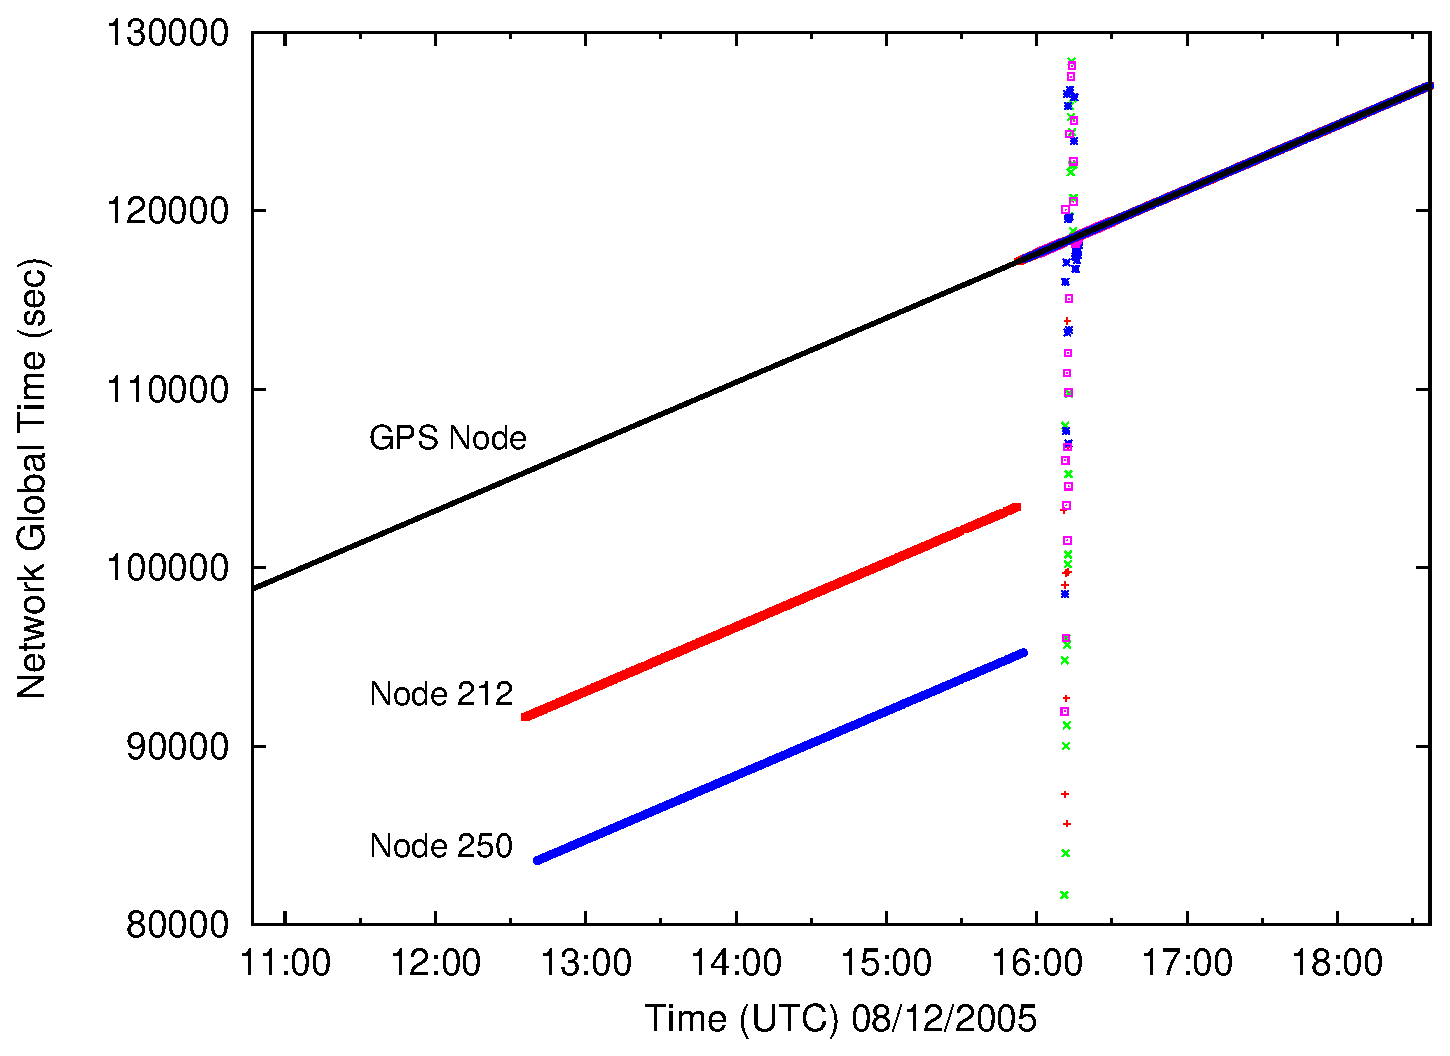
\includegraphics[width=\hsize]{./figs/OSDI2006/2006-FTSPInstability.eps}
\end{center} 
\caption{{\bf Example of FTSP instability observed during field deployment.}
The global time value reported by sensor nodes and the GPS node is plotted
against the time that the base station received the corresponding status
messages. All nodes are initially synchronized, but starting at 1230 GMT,
nodes 212~and~250 report incorrect global times for the next 4.5~hours. When
the nodes eventually resynchronize, the global timestamps of other nodes
initially experience some instability.}
\label{fig-FTSPInstability}
\end{figure}

Figure~\ref{fig-FTSPInstability} shows an example of the FTSP instability
observed in the field. The global time reported by two nodes suddenly jumps
off by several hours, and the nodes do not resynchronize until rebooted
4.5~hours later.  It turns out that two bugs combined to cause this problem.
First, it was discovered that the TinyOS clock driver would occasionally
return bogus local timestamps.\footnote{This bug was fixed in February 2006, several
months after our deployment.} Second, FTSP does not check the validity of
synchronization messages, so a node reading an incorrect value for its local
clock can corrupt the state of other nodes, throwing off the global time
calculation.

\begin{figure}[t]
\begin{center}
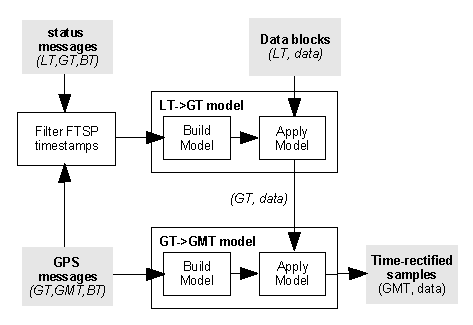
\includegraphics[width=0.8\hsize]{./figs/OSDI2006/2006-RectificationCartoon.eps}
\end{center}
\caption{{\bf Time rectification process overview.}}
\label{fig-rectificationcartoon}
\end{figure}

The failures of the time synchronization protocol made establishing the
correct GPS-based timestamp for each data sample extremely challenging.  To
do so, we developed a {\em time rectification} approach which filters and
remaps recorded timestamps to accurately recover timing despite these
failures. Figure~\ref{fig-rectificationcartoon} shows an overview of the
process.  The first step is to {\em filter} the global timestamps recorded
by each node, discarding bogus data. Second, we build a model mapping the
local time on each node to FTSP-based global time.  Third, we use the GPS
timestamp information to build a second model mapping FTSP time to GMT.
Finally, both models are applied to the timestamps recorded in each data
block producing a GMT time for each sample.

\subsubsection{Timestamp Filtering}
\label{subsection-filtering}

We begin by filtering out status messages appearing to contain incorrect
global timestamps. To do this, we correlate global timestamps from each node
against a common reference timebase and reject those that differ by more than
some threshold.  For this, we use the base station laptop's local time, which
is {\em only} used for filtering FTSP timestamps, not for establishing the
correct timing. The filtering process in is many ways similar to prior
work~\cite{paxson98calibrating,1028824} on detecting adjustments in
network-synchronized clocks.

We use the following abbreviations: {\em LT} is the local time of a node;
{\em GT} is the FTSP global time; {\em BT} is the base station's local time;
and {\em GMT} is the true GMT from the GPS signal.  The single GPS node
periodically sends a message logged by the base station consisting of the
triple {\em (GT, GMT, BT)}.  We use linear regression on this data to produce
a reference timebase mapping {\em BT} to {\em GT}.\footnote{We assume that
the global time reported by the GPS node is always correct; indeed, the
definition of ``global time'' is the FTSP time reported by the GPS node.}
Nodes periodically report their status through a heartbeat message, which
includes their local (LT) and global (GT) times, and for each node status
message logged by the laptop {\em (LT, GT, BT)}, we map {\em BT} to the
expected $\mathit{GT}_{\mathit{ref}}$ using the reference timebase. If $ \mid
\mathit{GT}_{\mathit{ref}} - \mathit{GT} \mid > \delta$, we discard the
status message from further consideration.  We use a threshold of $\delta =
1$~sec.  Although radio message propagation and delays on the base station
can affect the {\em BT} for each status message, a small rejection threshold
$\delta$ makes it unlikely that any truly incorrect FTSP timestamps pass the
filter. Indeed, of the 7.8\% of timestamps filtered out, the median {\em GT}
error was 8.1~hours.


\subsubsection{Timestamp Rectification}
\label{section-timerectification}

\begin{figure}[t]
\begin{center}
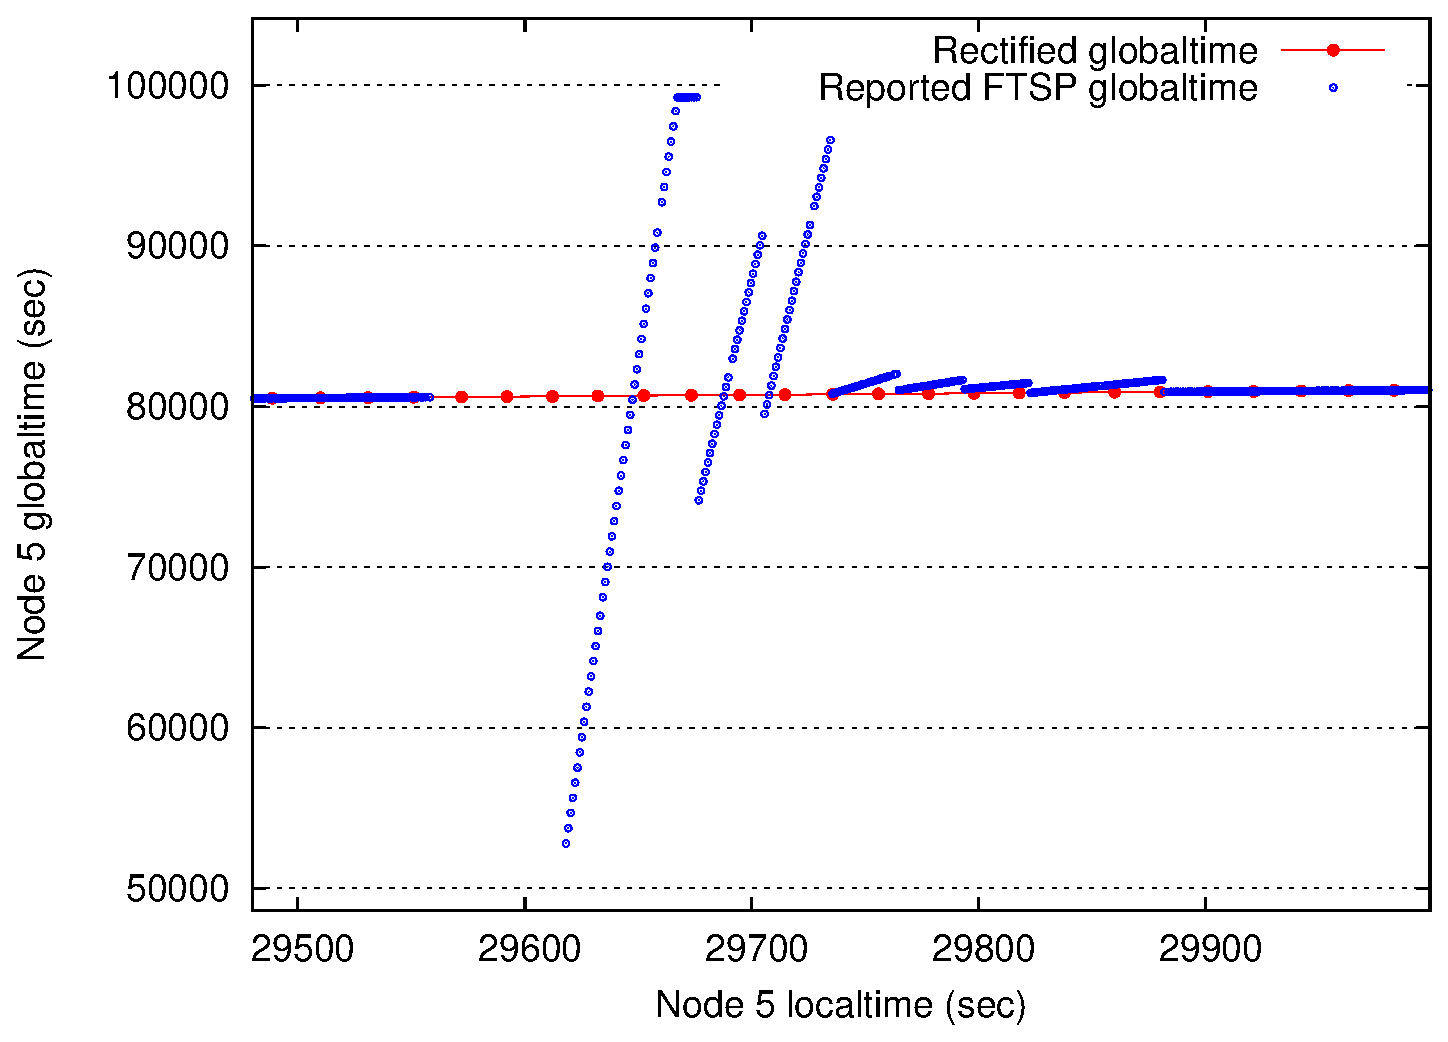
\includegraphics[width=\hsize]{./figs/OSDI2006/2006-TimingRectificationExample.eps}
\end{center}
\caption{{\bf Time rectification example.}
The raw (LT, GT) pairs collected from the node show that it experiences a
period of FTSP instability.  The time rectification process removes the
errant timestamps creating an accurate mapping between LT and GT created
using a linear regression on the remaining timestamps.}
\label{fig-timingrectificationexample}
\end{figure}

The goal of {\em time rectification} is to assign a GMT timestamp to each
sample in the recorded data. In order to do so, we build two models: one
mapping a node's local time to global time, and another mapping global time
to GMT. Figure~\ref{fig-timingrectificationexample} shows an example of this
process bridging a small local timing instability of the kind described
previously.

From those status messages that pass the filter, we build a piecewise linear
model mapping {\em LT} to {\em GT} using a series of linear regressions.
Models are constructed for each node separately, since local times vary
significantly between nodes.  Each regression spans up to 5~minutes of data
and we initiate a new regression if the gap between subsequent {\em (LT, GT)}
pairs exceeds 5~minutes.  Each interval must contain at least two valid
status messages to construct the model.  We take the {\em LT} value stored in
each data block and use this model to recover the corresponding {\em GT}
value.

The next step is to map global time to GMT. Each of the GPS node's status
messages contain a {\em (GT, GMT)} pair. As above, we build a piecewise
linear model mapping {\em GT} to {\em GMT}, and apply this model to the {\em
GT} values for each data block. Finally, we assign a GMT value to each sample
contained in the block, using linear interpolation between the GMT values
assigned to the first sample in each block.  This process makes no
assumptions about sampling rate, which varies slightly from node to node due
to clock drift.

\subsection{Evaluation}

Evaluating our time rectification process proved difficult, primarily because
we had no ground truth for the timing of the signals recorded in the field.
However, by reproducing the deployment conditions in the lab, we were able to
measure the accuracy of the recovered timing in a controlled setting.  In
addition, as described earlier, two GPS-synchronized data loggers were
colocated with our sensor network, providing us the opportunity to directly
compare our time-rectified signals with those recorded by conventional
instrumentation.

\subsubsection{Lab Experiments}

Our first validation took place in the lab. Feeding the output of a signal
generator to both a miniature version of our sensor network and to a
Reftek~130 data logger allowed us to directly compare the data between both
systems.  The miniature network consisted of a single sensor node, routing
gateway, and GPS receiver node. The same software was used as in the field
deployment. The Reftek~130 logs data to a flash memory card and timestamps
each sample using its own GPS receiver.

The results showed a consistent 15~ms offset between the time-rectified
signals recorded by the sensor node and the Reftek data logger.  We
discovered that this offset was due to delays introduced by the digital
filtering performed by the ADC on our sensor board (see
Sect.~\ref{sec-2005-board}). Adjusting for this delay resulted in an
indiscernible offset between the sensor node and Reftek signals. While this
experiment does not reproduce the full complexity of our deployed network, it
does serve as a baseline for validation.

In the second lab experiment, we set up a network of 7~sensor nodes in a
6-hop linear topology. The topology is enforced by software, but all nodes
are within radio range of each other, making it possible to stimulate all
nodes simultaneously with a radio message.  Each node samples data and sends
status messages using the same software as the field deployment. The FTSP
root node periodically transmits a beacon message. On reception of the
beacon, each node records the FTSP global timestamp of the message reception
time (note that reception of the beacon message is not limited by the
software-induced topology).  Because we expect all nodes to receive this
message at the same instant (modulo interrupt latency jitter) we expect the
FTSP time recorded at each node to be nearly identical. The FTSP root also
records the time that the beacon was transmitted, accounting for MAC delay.
The experiment ran for 34~hours, during which time FTSP experienced
instabilities similar to those seen during our deployment.

\begin{figure}
\caption{{\bf Timestamp errors in a 6-hop lab testbed.}
This table shows the 50th and 90th-percentile timing errors on both the raw
FTSP timestamps, and rectified timestamps.}
\vspace{0.2in}
\begin{center}
\begin{tabular}{lll}
\noalign{\smallskip}
                  & {\bf Raw error} & {\bf Rectified error} \\
\noalign{\smallskip}\svhline\noalign{\smallskip}
{\bf  1 hop}, 50th percentile & 1.52 ms & 1.42 ms \\ 
{\bf 1 hop}, 90th percentile & 9.86 ms & 6.77 ms \\
\noalign{\smallskip}\svhline\noalign{\smallskip}
{\bf 6 hops}, 50th percentile & 2.63 ms & 2.18 ms \\ 
{\bf 6 hops}, 90th percentile & 13.5 ms & 6.8 ms \\
\end{tabular}
\label{fig-time-rect-lab}
\end{center}
\end{figure}

This allows us to compare the {\em true} global time of each beacon message
transmission and the {\em apparent} global time on each receiving node, both
before and after subjecting the data to our time rectification process.  We
call the difference between the true and apparent times the {\em timestamp
error}. Figure~\ref{fig-time-rect-lab} shows the results for nodes one and
six hops away from the FTSP root.  After rectification, 99.9\% of the errors
for the one-hop node and 93.1\% of the errors for the six-hop node fall
within our 10~ms error envelope.

\subsubsection{Comparison with Broadband Station}

\begin{figure}[t]
\begin{center}
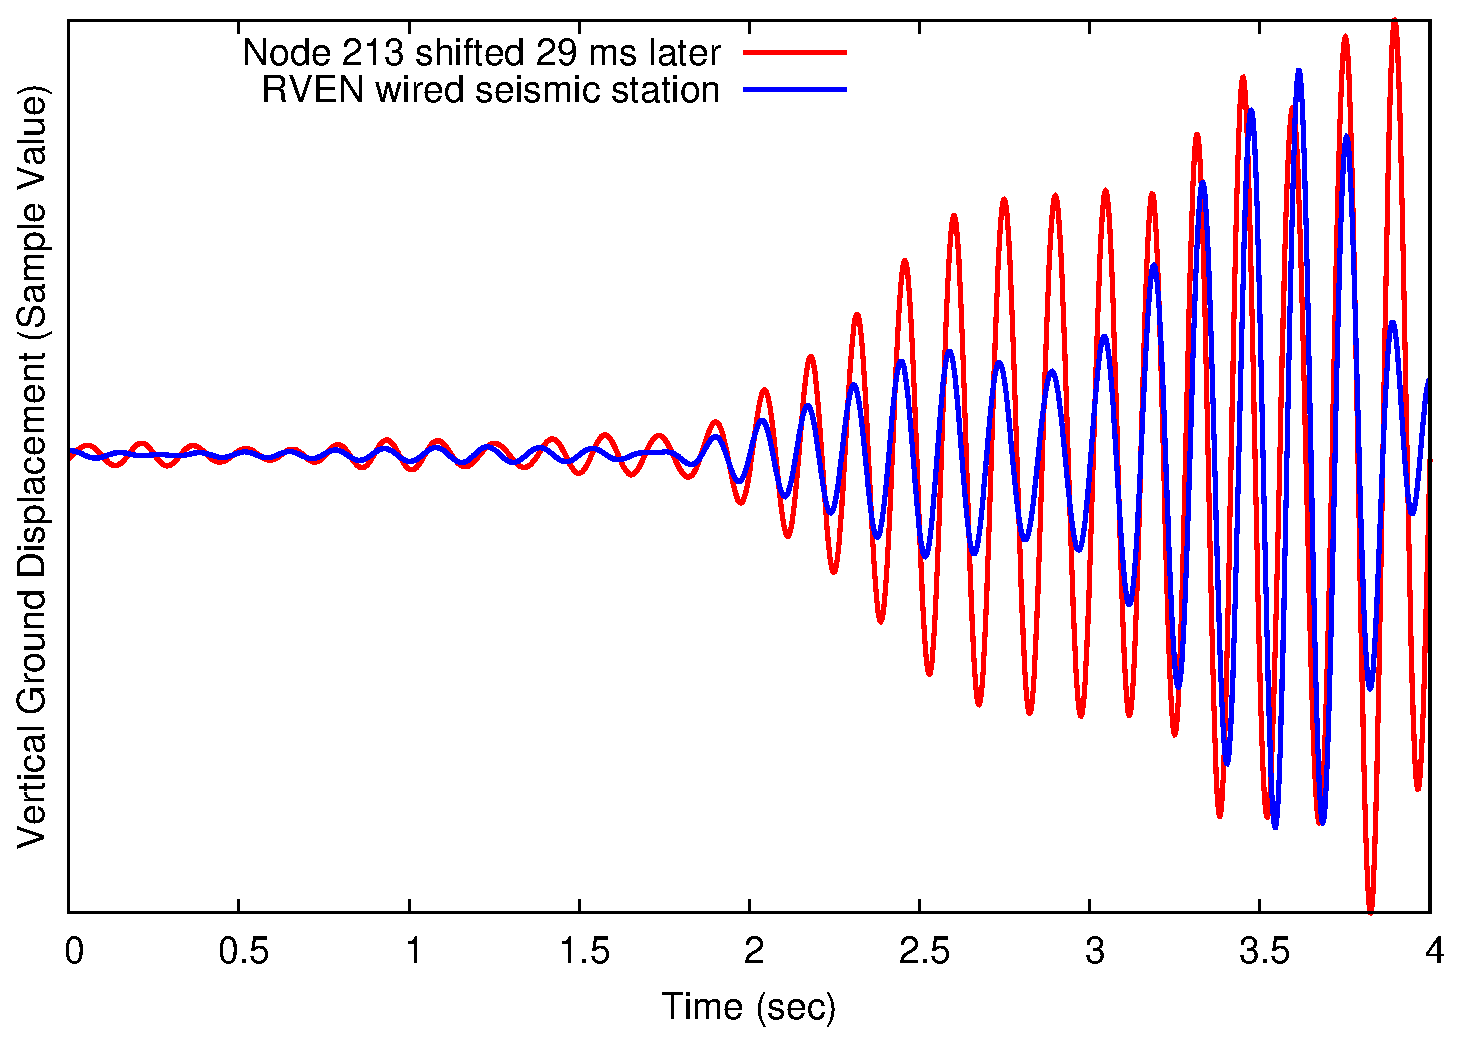
\includegraphics[width=\hsize]{./figs/OSDI2006/2006-reftekTimingExample.eps}
\end{center}
\caption{{\bf Comparison of RVEN and node~213 signals.}
This figure shows two seismic waves recorded by sensor node 213 and a
broadband seismometer located 56~m away. After time rectification, a 29~ms
time shift produces an excellent match.}
\label{fig-reftektimingexample}
\end{figure}

Although time rectification works well in the laboratory, it is also
necessary to evaluate its accuracy on the data collected during the field
deployment. For this purpose, we made use of one of the broadband seismometer
stations colocated with our sensor network. The RVEN (for ``Reventador
vent'') station was located 56~m from sensor node~213 (See
Fig.~\ref{fig-deployment-maps}(b)).  Given their
proximity, we would expect the seismic waveforms captured by both RVEN and
node~213 to be well correlated.  Some time shift between the two signals
would be expected: a seismic wave passing each station could be as slow as
1.5~km/sec, so the time lag between the signals could be as high as 37~ms.
However, due to differences in the seismometers and the placement and ground
coupling of the sensors, we would not expect perfectly correlated signals in
every case.

We identified 28~events recorded by both RVEN and node~213.  The data for
node~213 was time rectified as described earlier, and the RVEN data was
timestamped by the Reftek's internal GPS receiver.  We applied a bandpass
filter of 6--8~Hz to each signal to reduce sensor-specific artifacts. The
cross-correlation between the signals produces a set of of {\em lag times}
indicating possible time shifts between the two signals.  Due to the periodic
nature of the signals, this results in several lag times at multiples of the
dominant signal period. For each lag time, we visually inspected how well the
time-shifted signals overlapped and picked the best match by hand.

\begin{figure}[t]
\begin{center}
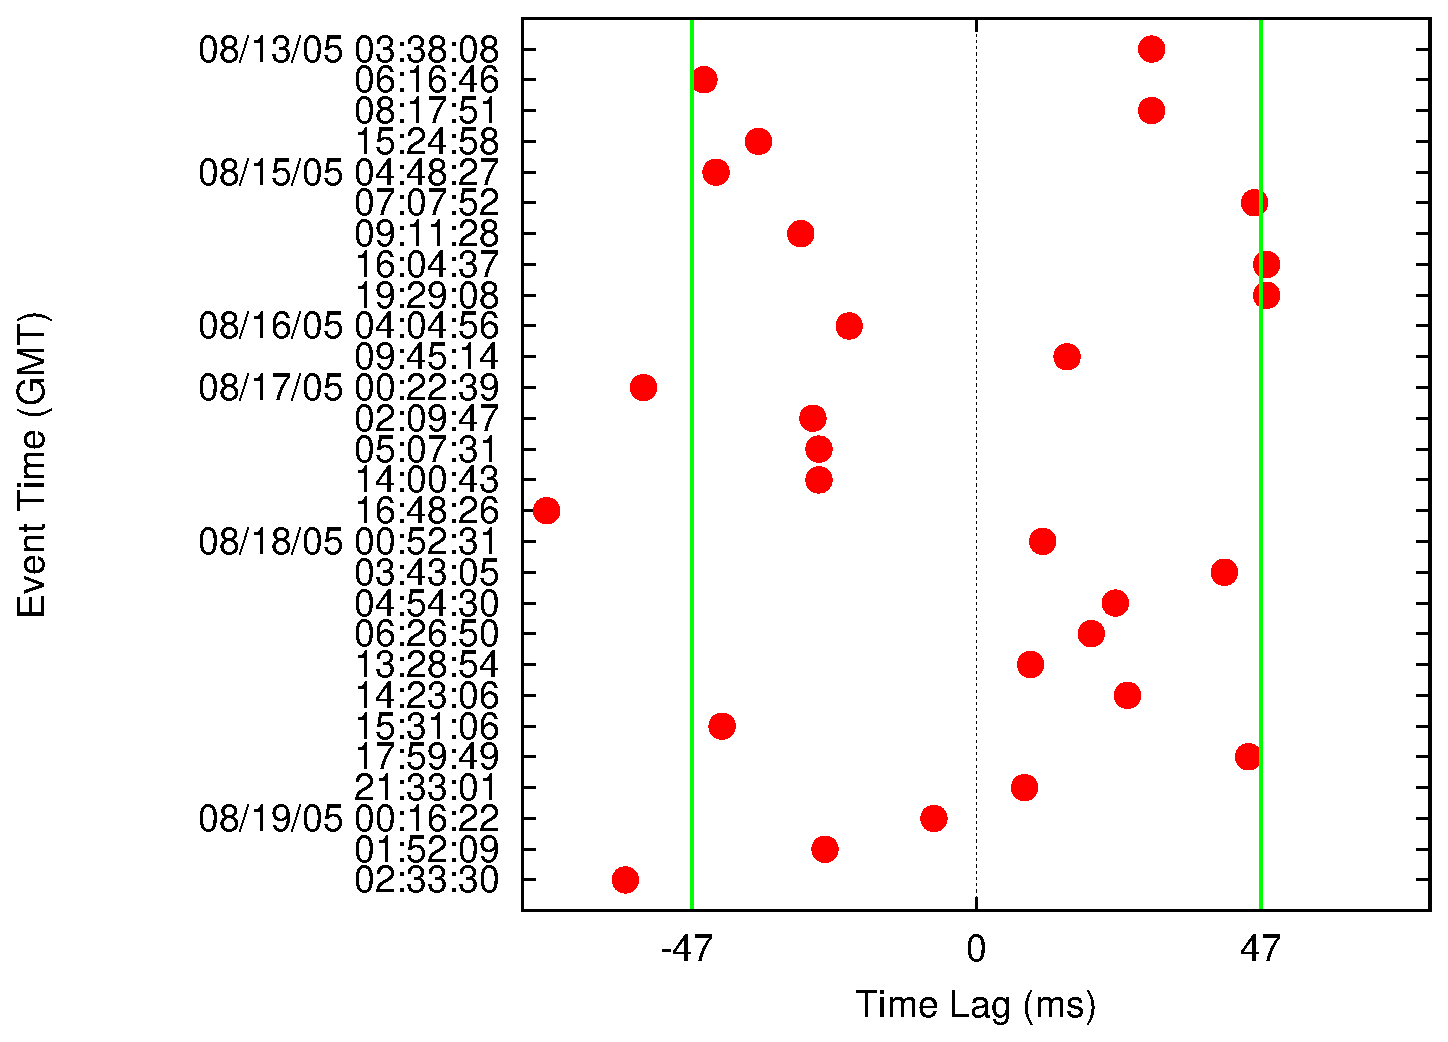
\includegraphics[width=\hsize]{./figs/OSDI2006/2006-TimingLags.eps}
\end{center}
\caption{{\bf Lag times between Node 213 and RVEN.}
The best lag time between the two stations is shown for 28 events.  best time
lag between the two stations is shown.  Most time shifts into the +/-~47~ms
window that we would expect given the distance between the two stations and
up to 10~ms of timing error.}
\label{fig-timinglags}
\end{figure}

Figure~\ref{fig-reftektimingexample} shows an example of this process that demonstrates
excellent correlation between the RVEN and node~213 signals with a 29~ms time
shift. Figure~\ref{fig-timinglags} shows a scatter plot of the best lag times
for all~28~events.  Of these, only 5~events fall outside of a $+/-$~47~ms
window defined by the distance between the stations ($+/-$~37~ms) and our
acceptable sampling error (10~ms). We have high confidence that our
time rectification process was able to recover accurate timing despite
failures of the FTSP protocol.

\subsection{Lessons Learned}

Overall there were many lessons we took away from our experience with data
timestamping.  First, due to the fact that development of the time
rectification technique took several months after the system teardown time,
we missed the critical window during which the scientific interest in our
data peaked.  Arriving in the field with an end-to-end solution ready to take
the output of our network and mold it into a form suitable for scientific
inspection would have been ideal, and is highly advisable for deployments
where scientist have clear datum quality expectations going in, as ours did.  

In addition to being unprepared for the issues we observed in the field, we
also did not think through the impacts of presenting half-baked data to the
seismologists we have been working with.  Particularly given our worries
about other parts of the system that did end up performing satisfactorily,
like the sampling board and driver (Sect.~\ref{subsec-signalhardware}), bulk
data transfer protocol and event detection mechanism, we were excited when
any signals at all showed up at the base station laptop. In our rush to
deploy the system we had not prepared an adequate data analysis and
visualization environment, and much of this was developed on-the-fly as the
deployment progressed. Due to this late and rushed development, none of the
initial tools did any of the post-hoc timing rectification that we eventually
had to perform in order to make the data suitable for scientific study.
Instead, we devised primitive tools allowing data from multiple stations to
be plotted together.

Unfortunately, these stacked plots were interpreted very differently
by the computer scientists and seismologists. To the computer scientists
these were evidence that the network was sampling data, detecting events and
successfully retrieving data using our bulk data-transfer protocol, namely
things were \textit{working}. Less concerned with the inner workings of our
system the seismologists appreciated little of this.  To them, these
poorly-synchronized signals were instead evidence that our signal timing was
extremely broken, a fear that persisted for some time after the deployment as
we worked hard together to rectify and validate the timestamps.  
The exposure of this intermediate data product to consumers unprepared for it
should serve as a cautionary tale about how much of the internal engineering
of a deployed WSN application to reveal externally.

Validating the timestamps on the data we did collect was also quite
frustrating and illustrates to what degree we were unprepared for the
severity of the timing challenge.  The several wired data loggers deployed
alongside our network all had attached GPS units providing extremely accurate
signal timing.  Had we thought to attach a single sensor both to one of our
wireless stations and, by simply splitting the output signal, to one of the
wired stations we could have easily cross-checked the timing with a known
ground truth (i.e. the identical signal).  In a remarkable oversight we never
thought to do this, meaning that we had no two identical inputs available to
reveal any inaccuracies in the timing information for the signals we
collected.  It would also have been useful to spend more time hardening FTSP
pre-deployment, and to have built in more logging and visibility into its
operation to help us at least have an idea, in situ, of how well it
was functioning.

While further work in this area would have been possible, our interests after
the 2005 deployment tended more in the direction of improving dataset
quality. Given our techniques to rectify the timestamps provided by FTSP were
already in place going forward, little additional work was done in this area.
In addition, FTSP has continued to be maintained and was canonicized as an
official mainline part of TinyOS in version 2.1.1 Given the importance of
accurate timestamping to many sensor network applications, certainly ones in
the scientific space, it is extremely encouraging that the sensor network
community has indicated its willingness to continue to test and maintain this
critical component.
